\subsection{Objetivo 3: Aplicación del filtro de Kalman para reducir el jitter y fusionar datos sensoriales}

La trilateración implementada previamente permitió obtener coordenadas de posición bidimensional del usuario, pero las mediciones resultaron demasiado inestables para su uso en una aplicación de producción. Las posiciones fluctuaban constantemente, incluso cuando el dispositivo permanecía estático, lo cual se debía al ruido intrínseco de los sensores UWB. Para mitigar este problema, se propuso combinar la información de la trilateración con los datos inerciales del acelerómetro del dispositivo móvil, aplicando un filtro de Kalman como técnica de fusión y suavizado de señales.

\subsubsection*{Fase 1: Recolección de datos crudos}

La lógica detrás de esta etapa era sencilla: si el acelerómetro indicaba que el usuario no se estaba moviendo, pero las coordenadas de la trilateración mostraban variaciones abruptas, entonces estas oscilaciones debían atribuirse al ruido de medición. Bajo este principio, se decidió capturar datos simultáneamente de ambos sistemas: las posiciones obtenidas mediante trilateración y las aceleraciones registradas por el acelerómetro.

Inicialmente se evaluó la posibilidad de calcular la posición únicamente a partir de los datos del acelerómetro, integrando dos veces la aceleración en el tiempo. Sin embargo, este enfoque se descartó rápidamente, ya que los errores de integración se acumulaban exponencialmente, provocando un crecimiento descontrolado en la magnitud del vector de velocidad y posición. En pruebas realizadas desplazándose en diagonal entre el origen y un punto máximo en el primer cuadrante, se observó que la magnitud del vector velocidad aumentaba de forma irreal, en lugar de mantenerse en valores compatibles con la velocidad promedio de una persona caminando (Figura~\ref{fig:velocidad}). 

% Ejemplo de cómo insertar esa gráfica si la tienes:
\begin{figure}[H]
   \centering
   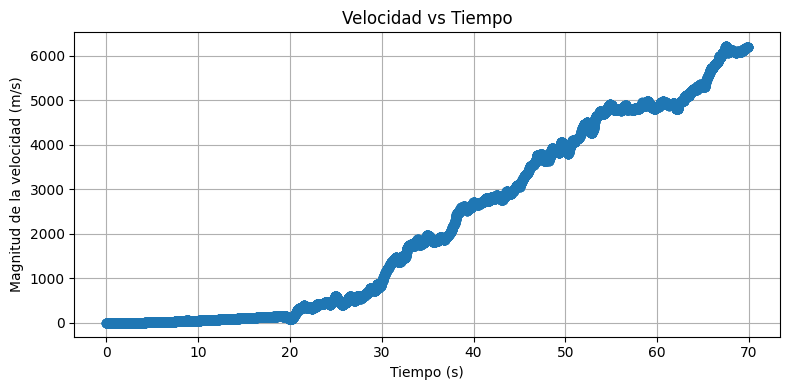
\includegraphics[width=0.8\textwidth]{images/accelerometer_velocity.png}
   \caption{Crecimiento de la velocidad al integrar los datos del acelerómetro para estimar la posición.}
   \label{fig:velocidad}
\end{figure}

Ante estos resultados, se optó por fusionar ambos conjuntos de datos mediante un filtro de Kalman. Este método no solo permite combinar información de distintas fuentes bajo un modelo dinámico de movimiento, sino que además suaviza el ruido de las mediciones. En la práctica, el filtro aprende progresivamente cómo se comporta el sistema, de modo que sus predicciones se vuelven más confiables que las propias mediciones crudas, las cuales solo se utilizan para realizar correcciones incrementales.

Para garantizar la reproducibilidad y evitar depender de pruebas físicas en cada iteración, se decidió capturar los datos crudos en un entorno controlado y analizarlos de forma simulada. Los datos fueron recolectados en el mismo cuarto rectangular utilizado para las pruebas de trilateración, desplazándose nuevamente en diagonal entre el origen y el primer cuadrante. Se almacenaron tanto las posiciones estimadas como las lecturas del acelerómetro en un archivo de texto con el siguiente formato:

\begin{verbatim}
Time: 1750964200.546540, Accel: x:-0.002765, y:-0.004459, z:-0.000987
Timestamp: 1750964200.603205, Position: Coordinate(x: 1.0589412, y: -0.8869535, z: 0.0)
\end{verbatim}

Dado que el archivo también contenía otros registros de la aplicación, fue necesario desarrollar un script de limpieza y parseo en Python, encargado de ordenar los datos cronológicamente y normalizar los formatos de tiempo y magnitud antes de alimentar la simulación del filtro de Kalman.

\subsubsection*{Fase 2: Implementación y ajuste del filtro de Kalman}

La simulación del filtro de Kalman se desarrolló inicialmente en Python, lo que permitió experimentar rápidamente con los hiperparámetros y evaluar los resultados visualmente. Antes de aplicar el filtro, se calculó la varianza de los datos crudos con el fin de estimar los valores iniciales de ruido de medición ($R$) y ruido del proceso ($Q$), fundamentales en el ajuste del filtro.

\begin{figure}[H]
    \centering
    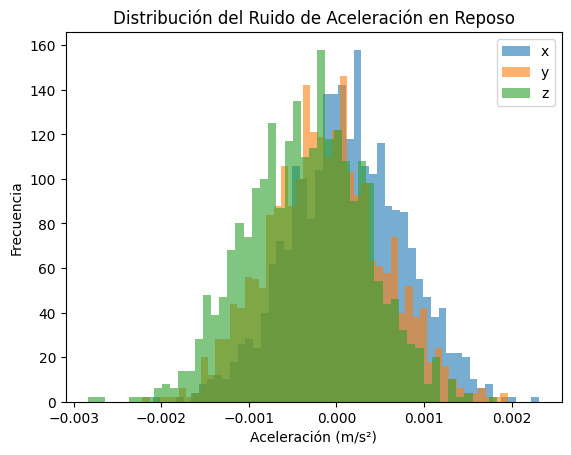
\includegraphics[width=0.75\textwidth]{images/accelerometer_distribution.png}
    \caption{Distribución del acelerómetro en reposo registrada mediante \textit{CoreMotion}. Los tres ejes presentan una varianza mínima, consistente con un estado de inmovilidad del dispositivo.}
    \label{fig:accelerometer_distribution}
\end{figure}

La varianza de las lecturas del acelerómetro en reposo fue extremadamente baja:

\[
\text{Var}_{acc} = [4.16\times10^{-7}, 4.33\times10^{-7}, 4.52\times10^{-7}]
\]


\begin{figure}[H]
    \centering
    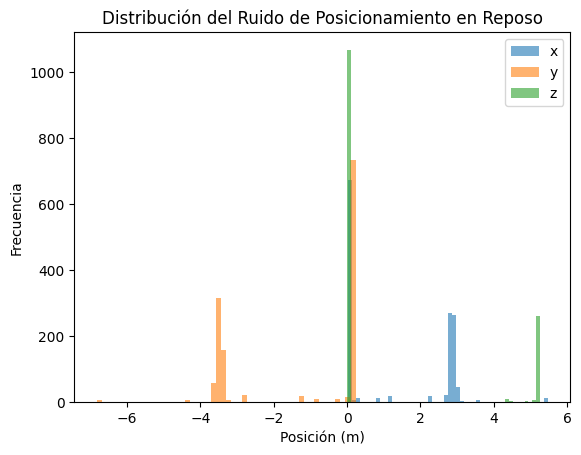
\includegraphics[width=0.75\textwidth]{images/kalman_position_distribution.png}
    \caption{Distribución de la posición estimada mediante trilateración en reposo. Se observan los tres ejes superpuestos.}
    \label{fig:kalman_position_distribution}
\end{figure}

Mientras que la varianza de los datos de posicionamiento obtenidos por trilateración resultó significativamente mayor:

\[
\text{Var}_{pos} = [2.02, 3.23, 4.40]
\]

El eje $z$ presentó una varianza más elevada debido a la naturaleza arbitraria de su cálculo (recordando que no siempre se encontraba una solución real al sistema, y en caso contrario se asignaba $z=0$). Esta diferencia era esperada, ya que el sistema no buscaba exactitud en $z$, sino estabilidad en el plano $x,y$.

Aunque los valores anteriores ofrecían una referencia inicial, se observó que las condiciones estáticas del acelerómetro subestimaban la varianza real durante el movimiento. Por ello, los hiperparámetros del filtro se determinaron finalmente de forma empírica, ajustándolos iterativamente hasta lograr un equilibrio entre respuesta rápida y suavizado efectivo.

El resultado se validó mediante la comparación visual entre la magnitud del vector de posición filtrado y no filtrado a lo largo del tiempo. 

Para ilustrar de manera más intuitiva el efecto del filtro de Kalman sobre el movimiento, se generó una trayectoria diagonal del usuario dentro del entorno de prueba. La Figura~\ref{fig:trajectory_comparison} muestra en el mismo plano la posición estimada con y sin filtrado, permitiendo observar claramente cómo el filtro suaviza los desplazamientos y reduce los saltos erráticos presentes en los datos crudos.

\begin{figure}[H]
    \centering
    % Subfigura 1: sin filtro
    \begin{subfigure}[b]{0.48\textwidth}
        \centering
        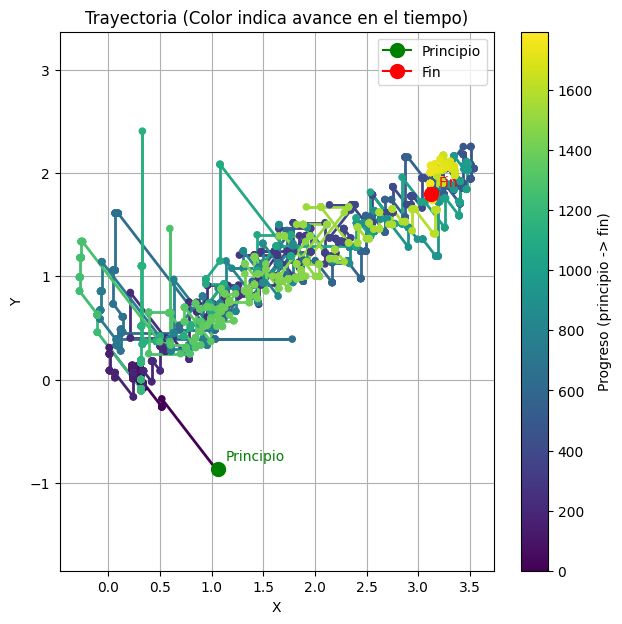
\includegraphics[width=\textwidth]{images/trajectory_unfiltered.png} % <-- ruta de la imagen sin filtro
        \caption{Trayectoria sin filtro de Kalman}
        \label{fig:trajectory_no_filter}
    \end{subfigure}
    \hfill
    % Subfigura 2: con filtro
    \begin{subfigure}[b]{0.48\textwidth}
        \centering
        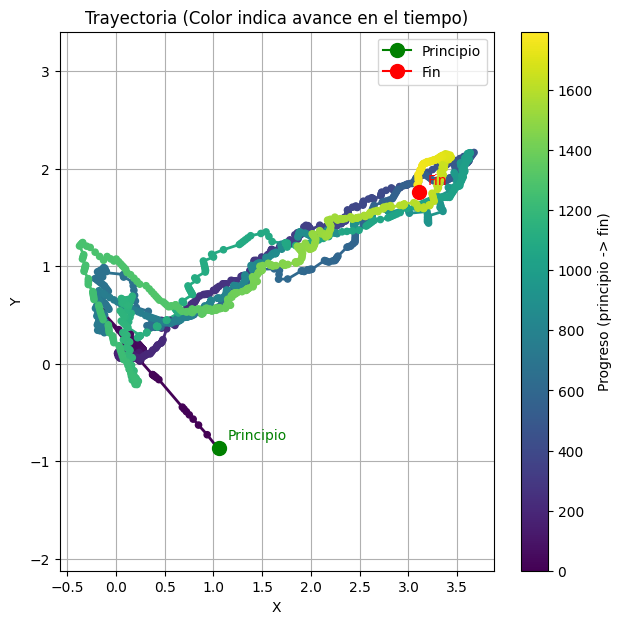
\includegraphics[width=\textwidth]{images/trajectory_filtered.png} % <-- ruta de la imagen con filtro
        \caption{Trayectoria con filtro de Kalman}
        \label{fig:trajectory_filtered}
    \end{subfigure}
    \caption{Comparación de la trayectoria diagonal del usuario en movimiento. La trayectoria filtrada muestra reducción de jitter y mayor suavidad respecto a la señal sin filtrar.}
    \label{fig:trajectory_comparison}
\end{figure}

Mientras la señal original mostraba un patrón ruidoso con picos abruptos (Figura~\ref{fig:jitter}), la señal filtrada exhibía una forma sinusoidal limpia y continua (Figura~\ref{fig:kalman}), reflejando el movimiento diagonal esperado.

% Ejemplo de cómo insertar las figuras:
\begin{figure}[H]
   \centering
   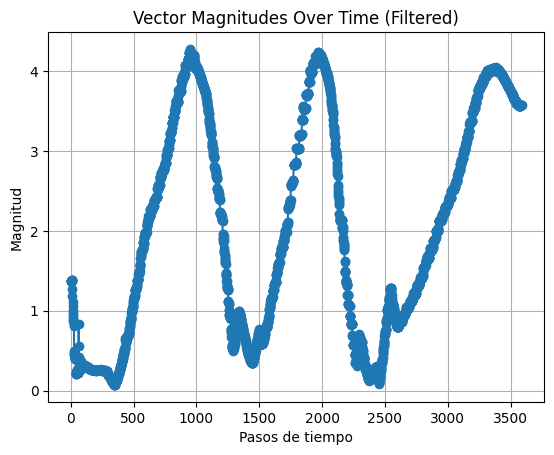
\includegraphics[width=0.8\textwidth]{images/filtered.png}
   \caption{Magnitudes de posición filtradas con Kalman.}
   \label{fig:kalman}
\end{figure}

\subsubsection*{Fase 3: Migración a Swift y refactorización arquitectónica}

Una vez calibrado el filtro en Python, se procedió a su implementación en Swift dentro del plugin nativo. En este punto fue necesario realizar una refactorización completa de la arquitectura del sistema, que hasta ese momento había sido utilizada únicamente como entorno experimental. 

El nuevo diseño adoptó el patrón de delegación (\textit{delegate pattern}) para desacoplar los módulos principales del sistema: gestión de sensores UWB, adquisición de datos inerciales y procesamiento de posición. Esta modularización mejoró la legibilidad del código y facilitó la extensión futura del sistema a otras plataformas.

La arquitectura final se estructuró en torno a tres componentes principales:
\begin{itemize}
    \item \textbf{UWBManager}: encargado de gestionar la conexión y actualización de distancias provenientes de los sensores UWB.
    \item \textbf{AccelerometerManager}: responsable de recolectar y transmitir las lecturas del acelerómetro usando \textit{CoreMotion}.
    \item \textbf{PositionCoordinator}: módulo central que fusiona las fuentes de datos aplicando la trilateración y el filtro de Kalman, devolviendo las coordenadas finales del usuario.
\end{itemize}

Estos módulos operan en un hilo secundario dedicado, con el fin de no bloquear el \textit{main thread} responsable de la interfaz gráfica. La decisión de mantener todo el procesamiento de localización en un solo hilo secundario obedeció al deseo de evitar sobrecargas por sincronización o calendarización, dado que el rendimiento observado era suficiente para un procesamiento en tiempo real.

% Diagrama de la arquitectura:
\begin{figure}[H]
   \centering
   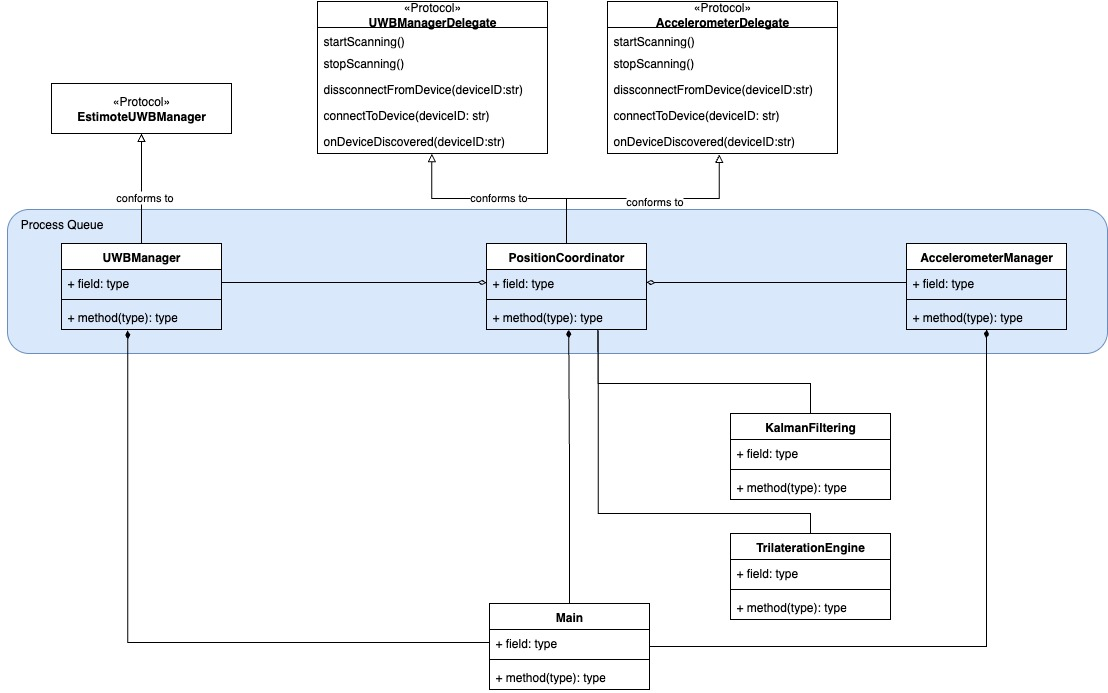
\includegraphics[width=0.8\textwidth]{images/Arch.jpg}
   \caption{Arquitectura final del sistema tras la integración del filtro de Kalman.}
   \label{fig:architecture}
\end{figure}

% \subsubsection*{Discusión de resultados}

% El uso del filtro de Kalman permitió reducir de manera sustancial las oscilaciones erráticas observadas en las posiciones calculadas por trilateración. La combinación de las fuentes de datos logró un posicionamiento más coherente, con trayectorias suaves y físicamente plausibles. Aunque el filtro introduce un pequeño retardo inherente al proceso de predicción y corrección, este resultó imperceptible en la experiencia del usuario dentro de la aplicación de realidad aumentada.

% En conjunto, esta etapa demostró que el filtro de Kalman no solo mejora la estabilidad de la señal, sino que también posibilita la integración robusta entre sensores UWB y acelerómetros en un entorno móvil. La correcta implementación y calibración de este modelo constituyó un paso esencial hacia un sistema de localización en tiempo real funcional y confiable.
